\subsection{构建阀体三维模型}
\begin{procedure}
\item 切换视图方向为西南等轴测。
\item 旋转产生孔实体。

旋转产生水平孔实体,其结果如图\ref{fig:fatisolid1} 所示。
\begin{lstlisting}
|命令: REVOLVE|
|当前线框密度:  ISOLINES=4,闭合轮廓创建模式 = 实体|
|选择要旋转的对象或 [模式(MO)]: 找到 1 个|
|选择要旋转的对象或 [模式(MO)]: 找到 1 个,总计 2 个|
|选择要旋转的对象或 [模式(MO)]: 找到 1 个,总计 3 个|
|选择要旋转的对象或 [模式(MO)]: 找到 1 个,总计 4 个|
|选择要旋转的对象或 [模式(MO)]: 找到 1 个,总计 5 个|
|选择要旋转的对象或 [模式(MO)]: 找到 1 个,总计 6 个|
|选择要旋转的对象或 [模式(MO)]: 找到 1 个,总计 7 个|
|选择要旋转的对象或 [模式(MO)]:|
|指定轴起点或根据以下选项之一定义轴 [对象(O)/X/Y/Z] $<$对象$>$:|
|指定轴端点:|
|指定旋转角度或 [起点角度(ST)/反转(R)/表达式(EX)] $<$360$>$:|
\end{lstlisting}
\begin{figure}[htbp]
\centering
\subfloat[]{\label{fig:fatisolid1}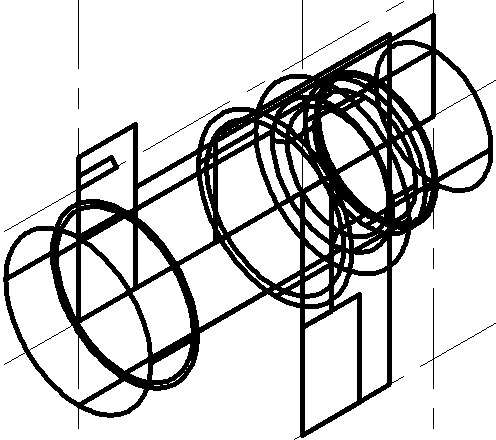
\includegraphics[scale=0.31]{fatisolid1.png}}\hspace{30pt}
\subfloat[]{\label{fig:fatisolid2}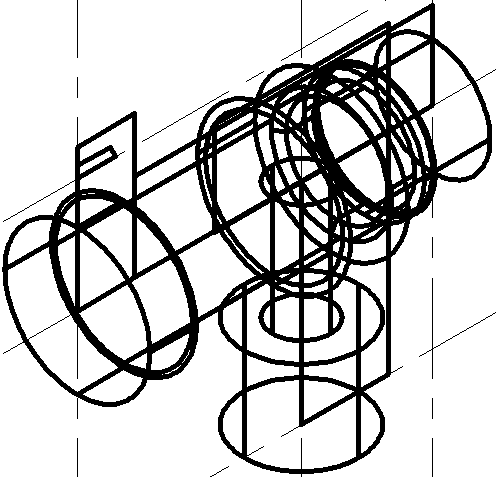
\includegraphics[scale=0.31]{fatisolid2.png}}\\
\subfloat[]{\label{fig:fatisolid3}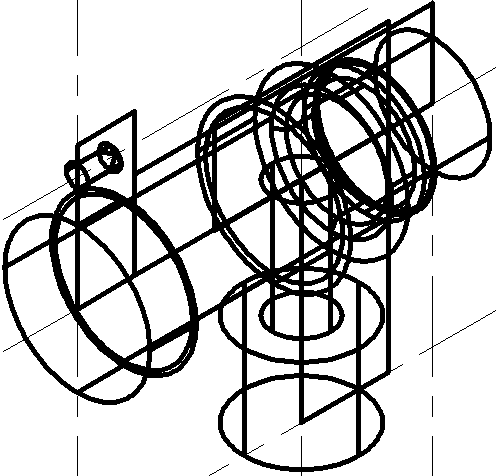
\includegraphics[scale=0.31]{fatisolid3.png}}\hspace{30pt}
\subfloat[]{\label{fig:fatisolid4}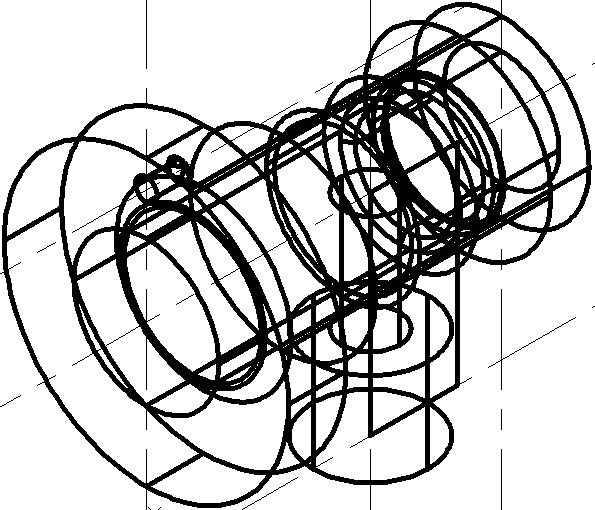
\includegraphics[scale=0.3]{fatisolid4.png}}
\caption{阀体三维模型构建过程一}
\end{figure}
旋转产生垂直孔实体,其结果如图\ref{fig:fatisolid2}所示。
\begin{lstlisting}
|命令: REVOLVE|
|当前线框密度:  ISOLINES=4,闭合轮廓创建模式 = 实体|
|选择要旋转的对象或 [模式(MO)]: 找到 1 个|
|选择要旋转的对象或 [模式(MO)]: 找到 1 个,总计 2 个|
|选择要旋转的对象或 [模式(MO)]:|
|指定轴起点或根据以下选项之一定义轴 [对象(O)/X/Y/Z] $<$对象$>$:|
|指定轴端点:|
|指定旋转角度或 [起点角度(ST)/反转(R)/表达式(EX)] $<$360$>$:|
\end{lstlisting}
旋转产生$M8$螺孔实体,其结果如图\ref{fig:fatisolid3}所示。
\begin{lstlisting}
|命令: REVOLVE|
|当前线框密度:  ISOLINES=4,闭合轮廓创建模式 = 实体|
|选择要旋转的对象或 [模式(MO)]: 找到 1 个|
|选择要旋转的对象或 [模式(MO)]:|
|指定轴起点或根据以下选项之一定义轴 [对象(O)/X/Y/Z] $<$对象$>$:|
|指定轴端点:|
|指定旋转角度或 [起点角度(ST)/反转(R)/表达式(EX)] $<$360$>$:|
\end{lstlisting}
旋转产生水平阀体实体,其结果如图\ref{fig:fatisolid4}所示。
\begin{lstlisting}
|命令: REVOLVE|
|当前线框密度:  ISOLINES=4,闭合轮廓创建模式 = 实体|
|选择要旋转的对象或 [模式(MO)]: 找到 1 个|
|选择要旋转的对象或 [模式(MO)]: 找到 1 个,总计 2 个|
|选择要旋转的对象或 [模式(MO)]:|
|指定轴起点或根据以下选项之一定义轴 [对象(O)/X/Y/Z] $<$对象$>$:|
|指定轴端点:|
|指定旋转角度或 [起点角度(ST)/反转(R)/表达式(EX)] $<$360$>$:|
\end{lstlisting}
\begin{figure}[htbp]
\centering
\subfloat[]{\label{fig:fatisolid5}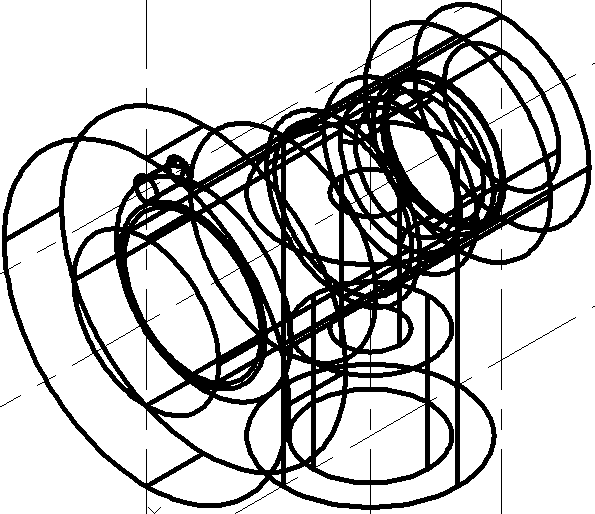
\includegraphics[scale=0.35]{fatisolid5.png}}\hspace{30pt}
\subfloat[]{\label{fig:fatisolid6}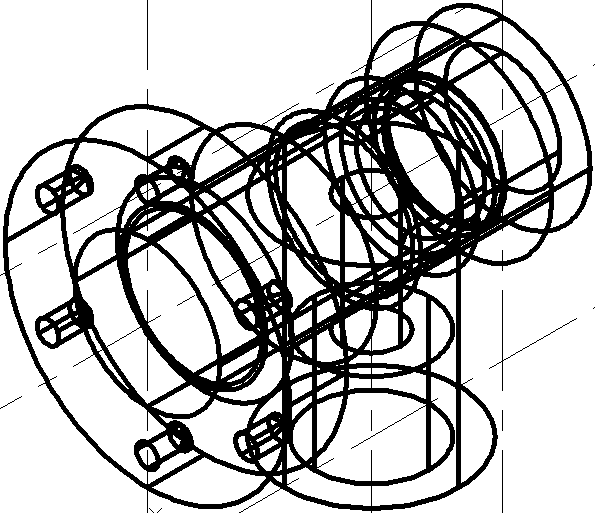
\includegraphics[scale=0.35]{fatisolid6.png}}\\
\subfloat[]{\label{fig:fatisolid7}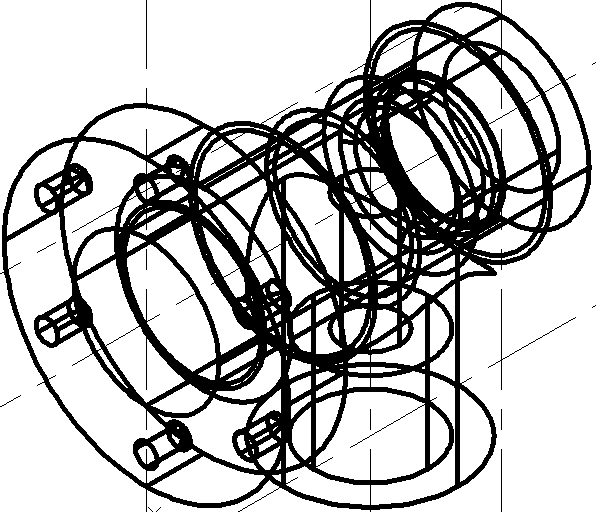
\includegraphics[scale=0.35]{fatisolid7.png}}\hspace{30pt}
\subfloat[]{\label{fig:fatisolid8}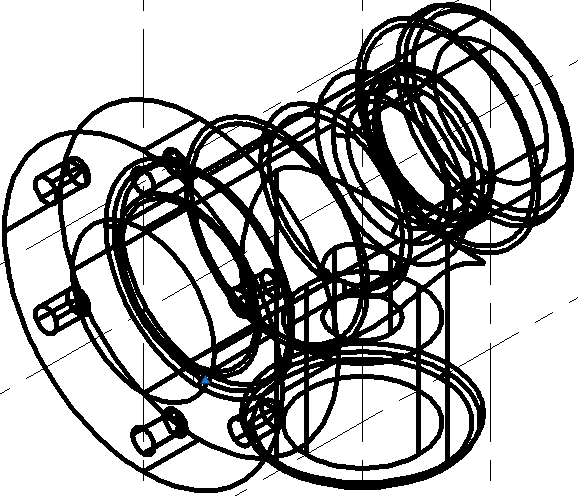
\includegraphics[scale=0.4]{fatisolid8.png}}
\caption{阀体三维模型构建过程二}
\end{figure}

旋转产生垂直阀体实体,其结果如图\ref{fig:fatisolid5}所示。
\begin{lstlisting}
|命令: REVOLVE|
|当前线框密度:  ISOLINES=4,闭合轮廓创建模式 = 实体|
|选择要旋转的对象或 [模式(MO)]: 找到 1 个|
|选择要旋转的对象或 [模式(MO)]:|
|指定轴起点或根据以下选项之一定义轴 [对象(O)/X/Y/Z] $<$对象$>$:|
|指定轴端点:|
|指定旋转角度或 [起点角度(ST)/反转(R)/表达式(EX)] $<$360$>$:|
\end{lstlisting}
\item 阵列生成6个$M8$螺孔,其结果如图\ref{fig:fatisolid6}。
\begin{lstlisting}
|命令: 3darray|
|选择对象: 找到 1 个|
|选择对象:|
|输入阵列类型 [矩形(R)/环形(P)]$<$矩形$>$:p|
|输入阵列中的项目数目: 6|
|指定要填充的角度 (+=逆时针, -=顺时针)$ <360>$:|
|旋转阵列对象? [是(Y)/否(N)] $<Y>$:|
|指定阵列的中心点:|
|指定旋转轴上的第二点:|
\end{lstlisting}
\item 合并阀实体。

将两个$\phi 64$圆柱体和$\phi 104$圆柱体合并为一个实体其结果如图\ref{fig:fatisolid7}所示。
\begin{lstlisting}
|命令: UNION|
|选择对象: 找到 1 个|
|选择对象: 找到 1 个,总计 2 个|
|选择对象: 找到 1 个,总计 3 个|
|选择对象:|
\end{lstlisting}

\item 生成阀体孔。
\begin{lstlisting}
|命令: SUBTRACT|
|选择要从中减去的实体、曲面和面域...|
|选择对象: 找到 1 个|
|选择对象:  选择要减去的实体、曲面和面域...|
|选择对象: 指定对角点: 找到 16 个|
|选择对象:|
\end{lstlisting}
\item 设置视觉样式为灰度,并将视图方向切换为东南等轴测。
\item 生成三维圆角

生成$R3$圆角,其结果如图\ref{fig:fatisolid8}所示。
\begin{lstlisting}
|命令: FILLETEDGE|
|半径 = 1.0000|
|选择边或 [链(C)/环(L)/半径(R)]: r|
|输入圆角半径或 [表达式(E)] $<$1.0000$>$: 3|
|选择边或 [链(C)/环(L)/半径(R)]:|
|选择边或 [链(C)/环(L)/半径(R)]:|
|选择边或 [链(C)/环(L)/半径(R)]:|
|选择边或 [链(C)/环(L)/半径(R)]:|
|已选定 3 个边用于圆角。|
|按 Enter 键接受圆角或 [半径(R)]:|
\end{lstlisting}
生成$R1$圆角。
\begin{lstlisting}
|命令: FILLETEDGE|
|半径 = 3.0000|
|选择边或 [链(C)/环(L)/半径(R)]: r|
|输入圆角半径或 [表达式(E)] $<$3.0000$>$: 1|
|选择边或 [链(C)/环(L)/半径(R)]:|
|选择边或 [链(C)/环(L)/半径(R)]:|
|选择边或 [链(C)/环(L)/半径(R)]:|
|已选定 2 个边用于圆角。|
|按 Enter 键接受圆角或 [半径(R)]:|
\end{lstlisting}
\item 生成三维倒角,其结果如图\ref{fig:fatisolid9}所示。

启动三维角命令的方法有:
\begin{itemize}
\item 键盘输入CHAMFEREDGE。
\item 点击【修改】中的【实体编辑】子菜单中的【倒角边】项。
\item 点击【实体编辑】工具栏中的【倒角边】图标
\includegraphics[scale=0.6]{chamferedge.png}。
\end{itemize}
生成$M42$水平螺孔倒角。
\begin{lstlisting}
|命令:CHAMFEREDGE|
|距离 1 = 2.0000,距离 2 = 4.0000|
|选择一条边或 [环(L)/距离(D)]: d|
|指定距离 1 或 [表达式(E)] $<$2.0000$>$:|
|指定距离 2 或 [表达式(E)] $<$4.0000$>$: 2|
|选择一条边或 [环(L)/距离(D)]:|
|选择同一个面上的其他边或 [环(L)/距离(D)]:|
|按 Enter 键接受倒角或 [距离(D)]:|
\end{lstlisting}
生成$M42$垂直螺孔倒角。
\begin{lstlisting}
|命令:  CHAMFEREDGE|
|距离 1 = 2.0000,距离 2 = 2.0000|
|选择一条边或 [环(L)/距离(D)]:|
|选择同一个面上的其他边或 [环(L)/距离(D)]:|
|按 Enter 键接受倒角或 [距离(D)]:|
\end{lstlisting}
生成$\phi 53$孔倒角。
\begin{lstlisting}
|命令:  CHAMFEREDGE|
|距离 1 = 2.0000,距离 2 = 2.0000|
|选择一条边或 [环(L)/距离(D)]:|
|选择同一个面上的其他边或 [环(L)/距离(D)]:|
|按 Enter 键接受倒角或 [距离(D)]:|
\end{lstlisting}
\begin{figure}[htbp]
\centering
\subfloat[]{\label{fig:fatisolid9}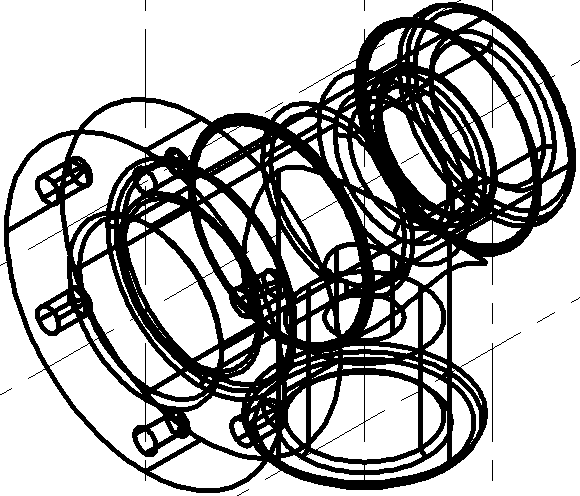
\includegraphics[scale=0.35]{fatisolid9.png}}\hspace{30pt}
\subfloat[]{\label{fig:fatisolid10}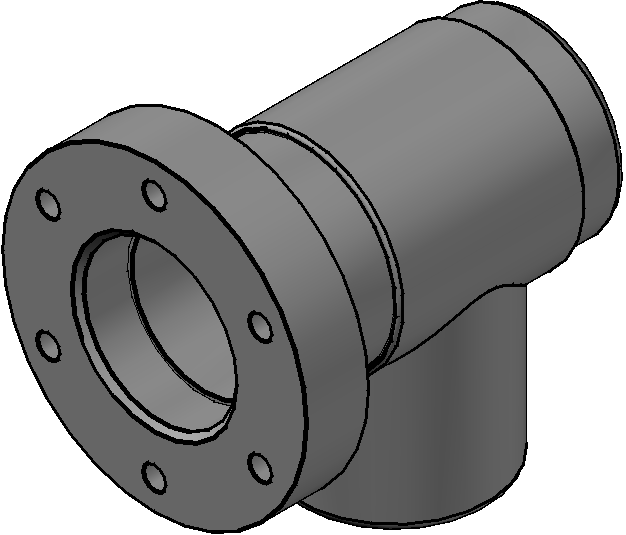
\includegraphics[scale=0.35]{fatisolid10.png}}
\caption{阀体三维模型构建过程三}
\end{figure}
\item 设置视觉样式为灰度,其结果如图\ref{fig:fatisolid10}所示。
\item 将阀体模型保存为“调压阀阀体立体图.dwg”。
\end{procedure}
\endinput